% !TeX spellcheck = en_US

\chapter{AR specific problems regarding realization}

\section{Hardware}
\label{sec:hardware}
As uFixit only provides the software solution for interactive manuals, the user is free to choose which kind of AR hardware he would like to choose for the application. To make the selection process easier, we first specify the requirements, that the hardware has to fulfill and then propose to possible hardware devices that are compatible with uFixit.

\subsection{Requirements}
Although there is no specific augmented reality hardware that is required to run uFixit manuals, a few requirements have to be fulfilled.

Firstly, the hardware has to be \textbf{mobile}, so that the user can take the instructions to the item he wants to repair. This is especially important if the item in question is too heavy to be moved, or is firmly mounted to its location. Therefore, the uFixit hardware has to be small and light enough to be carried around, and also has to assemble and disassemble quickly.

This also rules out head tracking systems for the augmented experience, which require the installation of tracking cameras around the user to follow his head movements. Instead, a high resolution \textbf{RGB camera} is used for the object detection and an optional \textbf{depth camera} provides the exact distance between the observed object and the uFixit hardware.

Another important factor is, that many repairing tasks, require both hands to be executed. Therefore, the augmented reality device has to be \textbf{worn on the head}, so that the user can see the instruction manual all the time, without holding the device in one hand. This also requires a \textbf{lightweight} hardware solution, as the whole weight is carried only by the head.

If the current step of the instruction set is completed by the user, the next step is selected by speech commands. Speech control is the only suitable way for navigating through an uFixit manual, because it requires no hand interaction and therefore lets the user concentrate on the task. This means, that the hardware also has to supply a \textbf{microphone} to pick up the user commands.

The last requirement, regarding the \textbf{computational power} of the device, is a not very restrictive. As uFixit essentially replays previously defined sequences of markers and overlays, the main computational effort lies in the real time object detection and to match those augmentations with the real world. This task is already executed by the hardware used in today’s mobile phones and therefore is not a limitation for the hardware selection process.

\subsection{Hardware Proposals}
Now we propose two already existing hardware solutions, which are guaranteed to be compatible with the uFixit application. 

The first one is the "Meta 2", a lightweight optical see through glass with an integraded 720p camera and a 3D depth sensor. It also has additional sensors for head movement tracking, which supports the optical camera tracking via sensor fusion. The downside is, that the "Meta 2" has no integrated processor and has to be connected to an Laptop. It also provides no microphone, which however is no problem, as the microphone can be connected to the required computer.
Other optical see though glasses are of course also possible candidates for uFixit, as long as they have at least a camera, which is HD-ready, microphone support and enough processing power for the application.
\begin{figure}[H]
		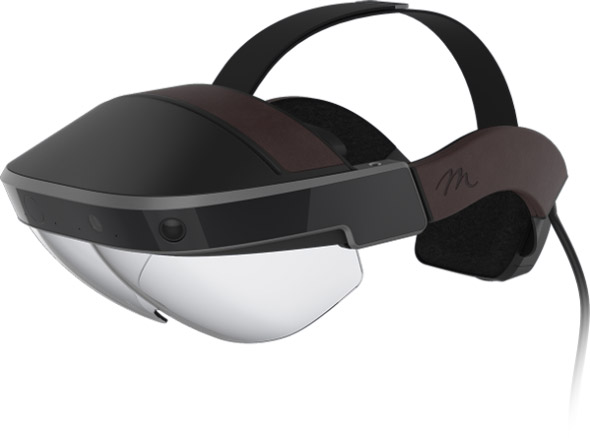
\includegraphics[width=0.66\textwidth]{../images/meta2.jpg}
		\centering
		\caption{Meta 2 - Augmented Reality Glasses}
		\label{fig:SWOT}
\end{figure}

The second class of supported hardware are mobile phones, especially in combination with projects like "Google Cardboard" or Samsung's "Gear VR", which transform the phones to augmented reality glasses. The big advantage of mobile phones is, that they are already very common, and therefore uFixit can be used  without spending extra money on additional hardware. Modern smart phones also meet the basic requirements for our application, as they already include high resolution cameras, sufficient computational power and a microphone for user input. We would also like to emphasize that devices, which are certified by Google's "Project Tango" are especially suited for uFixit, as those devices provide an additional depth camera for an even better user experience.
\begin{figure}[H]
		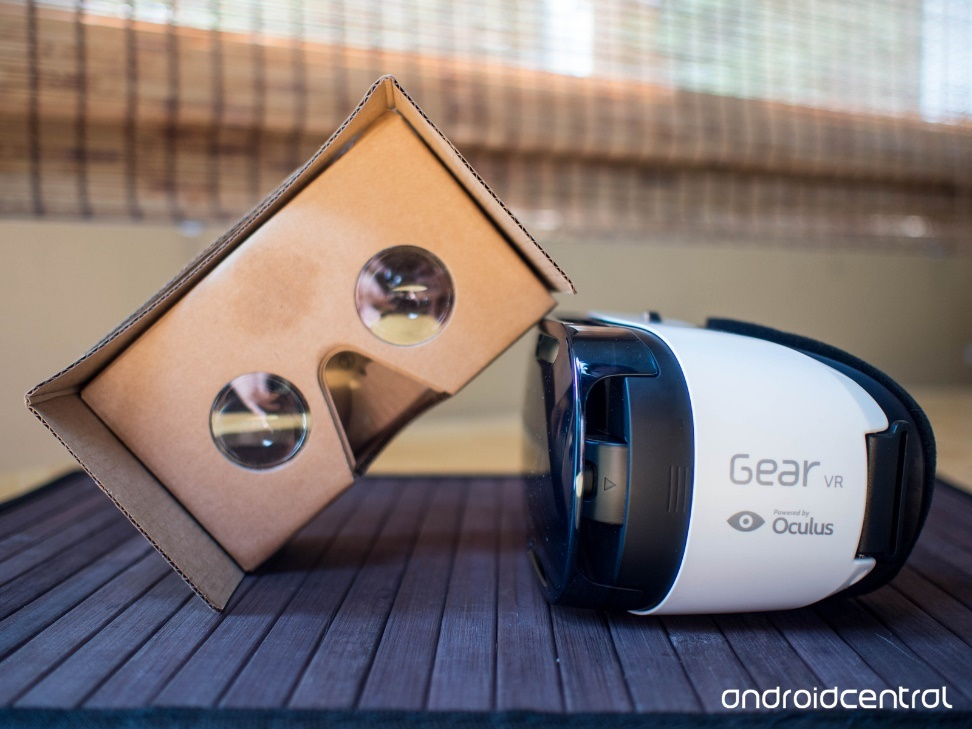
\includegraphics[width=0.66\textwidth]{../images/googleCarboard.jpg}
		\centering
		\caption{Google Cardboard and Gear VR}
		\label{fig:cardBoard}
\end{figure}
				

\section{Software}
\subsection{Computer Vison}
To provide the best augmented experience possible, it is essential that the virtual objects and annotations of the uFixit manual always remain at the same spatial position of the objects they are enhancing in the real world. The uFixit software provides two different approaches to find the right locations for the annotations.

The first one uses the RGB camera of the augmented reality glasses to detect the features of the items, that are visible to the camera view. The software is now tracking these features from frame to frame throughout the video stream and matches them to the systems internal,  virtual representation of the object. The system then uses the information about matched feature positions, to overlay the annotations provided by the manual onto the users view of the real world.

As uFixit is a platform for repairing broken or deformed parts, it might be impossible for the system to detect the features of the object in question. This is why it is also possible for the creator of the manuals to provide position for optional Fiducial Markers. The fixer prints these markers on paper and attaches them to specific locations of the broken item, as predefined by the creator of the manual. The big advantage of Fiducial Markers is, that compared to object features markers have a predefined shape and a limited set of colors. Therefore they are easier to recognize and to track by the system.
\begin{figure}[H]
		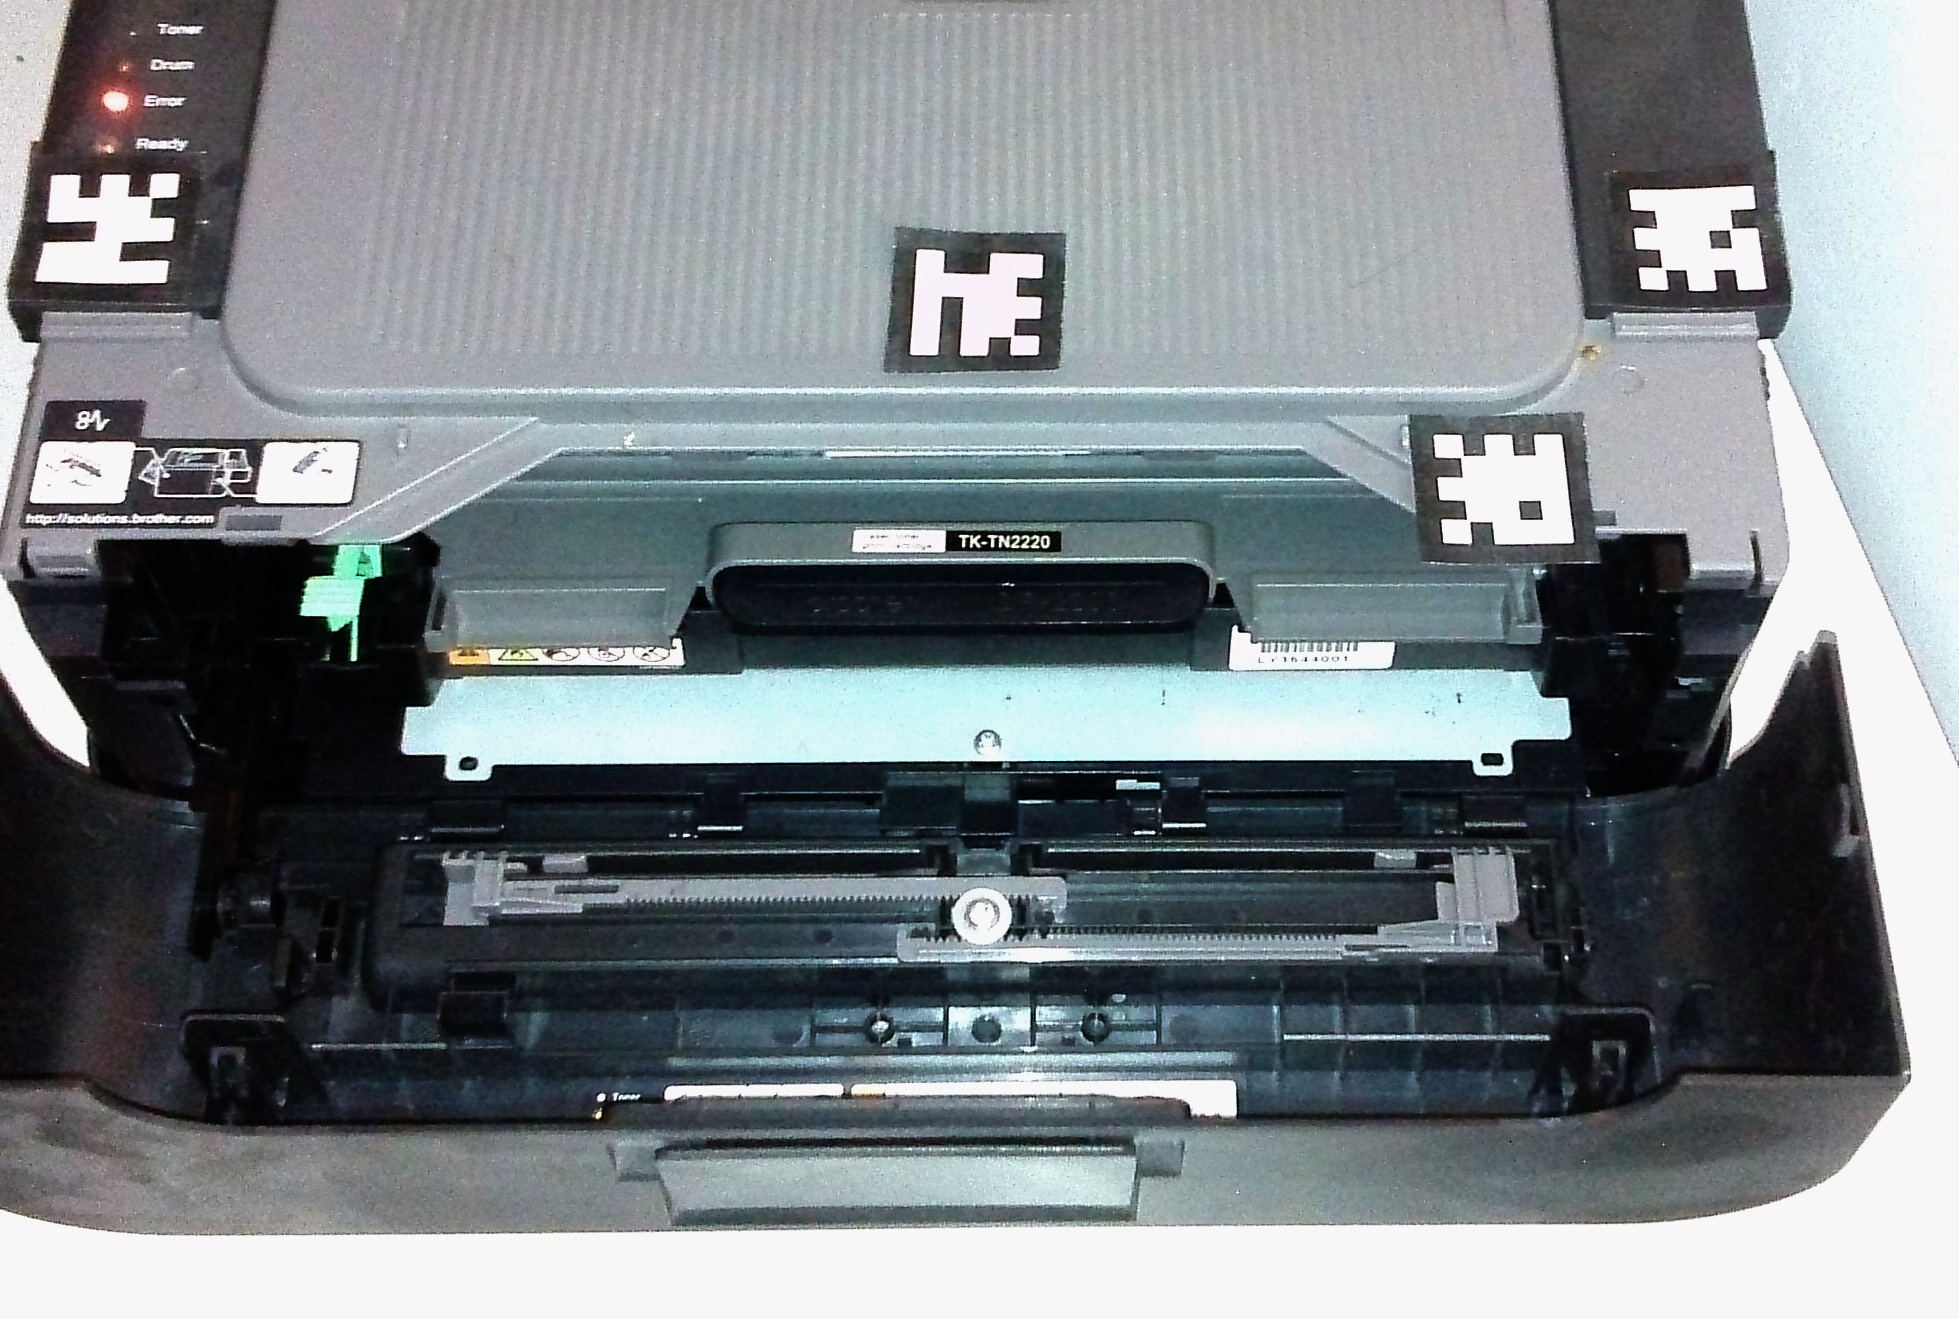
\includegraphics[width=0.66\textwidth]{../images/markerOnObject.jpg}
		\centering
		\caption{Printer with Fiducial Markers at specified positions}
		\label{fig:cardBoard}
\end{figure}

If an object is too small for markers to be placed on it, there is also the possibility of printing a big paper sheet with markers on its edges. The user then has to position the object he would like to repair at a certain position, centered on the sheet. This makes it possible for the system to show an augmentation of the object, by tracking the paper sheet with the object being at a certain position with a known offset to the markers.
\begin{figure}[H]
		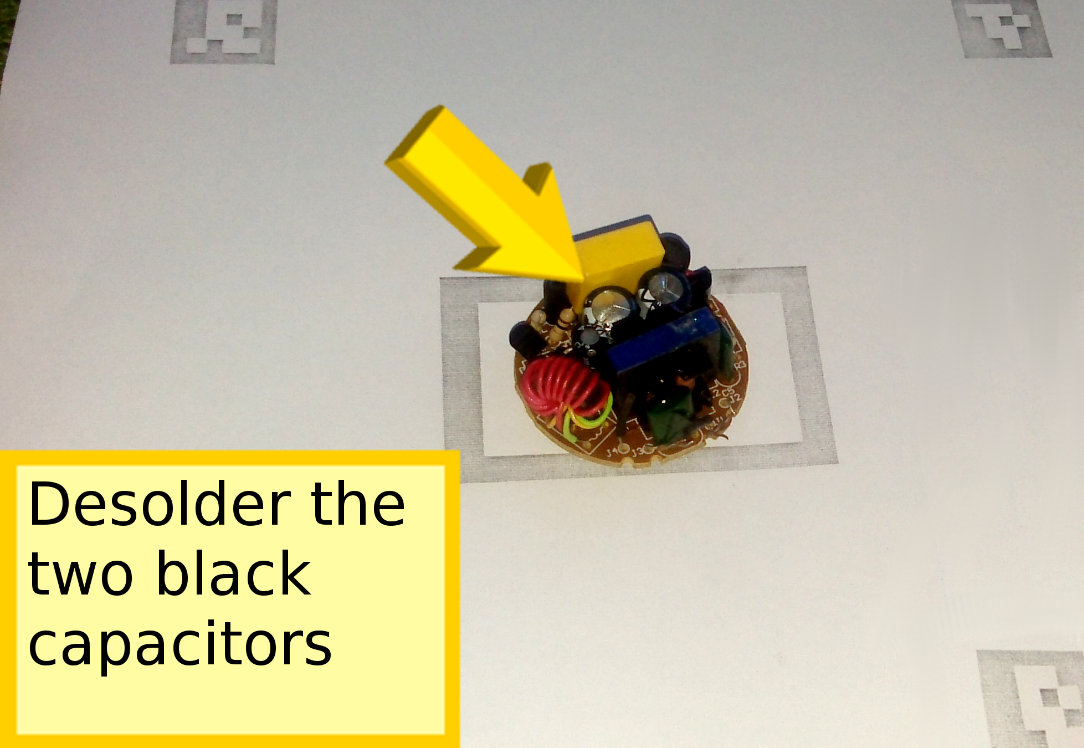
\includegraphics[width=0.66\textwidth]{../images/markerOnPaper.png}
		\centering
		\caption{Small object, centered between Fiducial Markers}
		\label{fig:cardBoard}
\end{figure}

As described in the hardware section \ref{sec:hardware}, uFixit also supports an optional depth camera. This adds the feature of occluded virtual elements to the system, as the additional depth information enables the application, to determine the exact distance between the watched item and the AR glasses. Therefore, if an virtual annotation is attached to the other side of the object, uFixit is able to temporarily hide this information from the user until the object is flipped around again. This feature helps the user to better understand the spatial relation of the virtual annotations and the real word object.
As this is an optional feature, the application also works without a depth sensor. The only drawback is, that all annotations of the current manual step then are visible the whole time, even if they should be occluded by the object.


\subsection{Manual creation (Manufacturer)}
Instead of shipping paper manuals with their product, uFixit provides an alternative solution for manufacturers. The big advantage of an digital manual is, that errors in the manual or information updated to the product do not require a reprint of the whole manual, but only an update of the uFixit database. Nowadays, industrial products are designed in CAD software like "Solidworks". These softwares packages also provide additional features like animation of the designed items (like rotating screws), creating semi transparent highlighting objects, or adding text objects for explanations. This is why uFixit provides an import interface for industrial instruction creators, that is able to import CAD projects and use them as a part of an uFixit manual. Each of the imported snippets then makes up one step of the final instruction set.

\begin{figure}[H]
		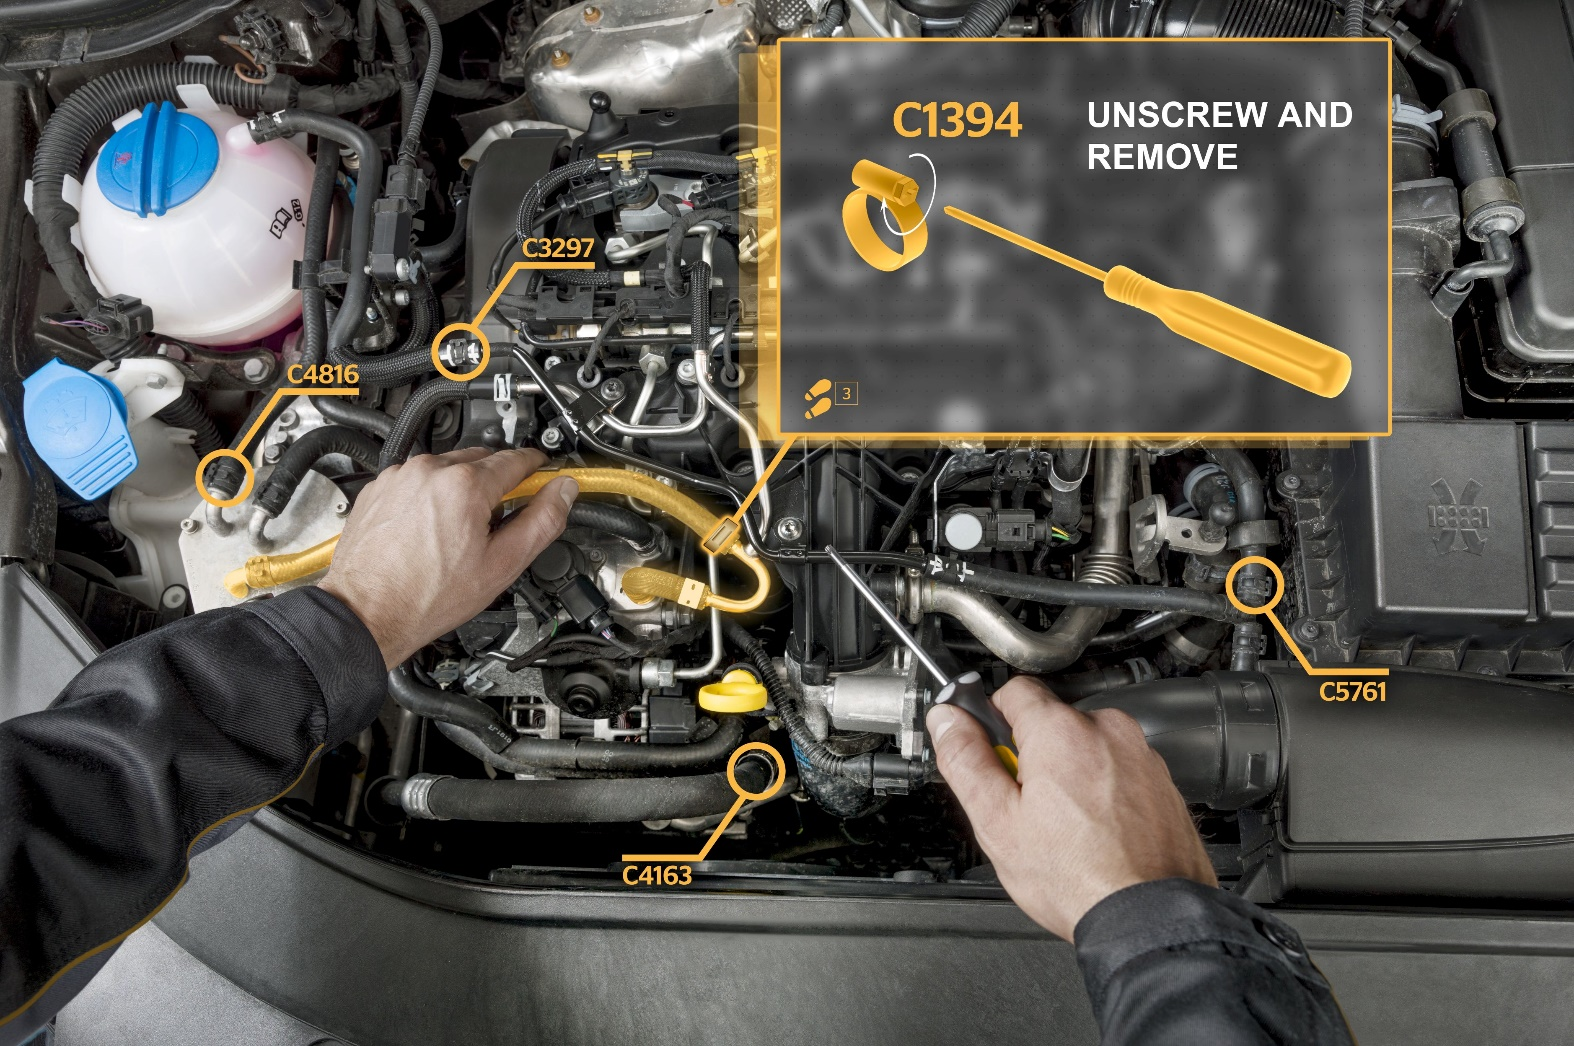
\includegraphics[width=0.66\textwidth]{../images/manufacturer.jpg}
		\centering
		\caption{Manufacturer created uFixit manual}
		\label{fig:cardBoard}
\end{figure}


\subsection{Manual creation (End User)}
Each uFixit user is also able to create own instruction sets and provide them to the community. For the creation, the same hardware is used as if following an manual, with the constraint that a depth camera is a requirement for the manual creation. It is required for the precise spatial registration of the manual annotations with the key features of the real world object. For each step of the instruction manual, there are the following annotations possibilities:

\begin{itemize}
\item Arrows
\item Text
\item Highlighting
\item Sketches
\end{itemize}

To annotate items, uFixit uses representations of the annotations in paper form. When paper templates are recognized by the camera, the software adds the corresponding virtual annotation object at the exact location of the paper template. 

\begin{figure}[H]
		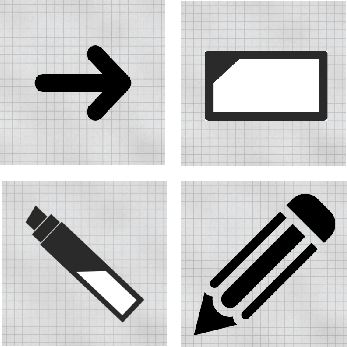
\includegraphics[width=0.66\textwidth]{../images/paperMarker.png}
		\centering
		\caption{Annotation templates}
		\label{fig:cardBoard}
\end{figure}

If for example, an arrow should be added to the current manual step, the user holds the piece of paper with the printed arrow symbol at the position, where the arrow should appear in the manual. 

\begin{figure}[H]
		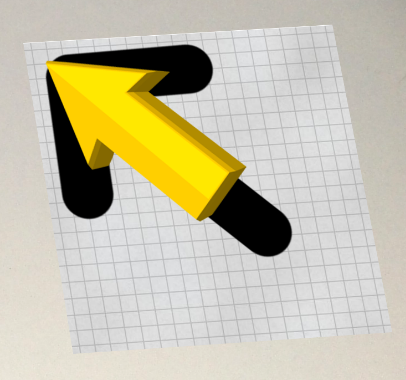
\includegraphics[width=0.66\textwidth]{../images/paperArrowAugmented.png}
		\centering
		\caption{Paper template with virtual annotation arrow}
		\label{fig:cardBoard}
\end{figure}

The position is then finalized by speech command ("Attach Here").

The text annotation is positioned in exactly the same way. The text is then filled in also using speech recognition.
Highlighting and sketches works in the way, that the manual creator moves the tip of the printed highlighter (or pen) at the start position of the annotation. Drawing begins after the "Start drawing" speech command. All locations at the highlighter/pen tip are then highlighted until the stop command is given.


\subsection{Live support}
In contrast to the static manuals, the uFixit live support focuses on quick and simple features. Writing annotation texts or creating animations simply takes too much time for the live scenario. This is why the live support limits the possibilities for augmentation to these four features:
\begin{itemize}
\item Arrows
\item Highlighting
\item Audio communication
\end{itemize}

In contrast to all other functions of uFixit, the expert providing live support uses a tablet or PC for the interaction. On the display, the live stream of the AR device camera is displayed. The expert now draws and positions the annotations using the touch screen or mouse onto the video.
Due to the visual object tracking by camera, the software is able to anchor the provided visual annotations at the location in space, where they were created. If the live support highlights specific locations of the camera view, these annotations remain with the object, even if the camera view changes.

To avoid scrawly drawings, due to the constantly changing camera view, the camera stream can be frozen. That means, that the annotations are drawn onto one image of the view, but are still updated in real time into the augmented view.
